\section{Mathematics}
\label{geometry}

\subsection{Schwarzschild metric}
The variation of action gives rise to the Euler-Lagrange equations
\begin{align}
\dfrac{\mathrm{d}}{\mathrm{d}\sigma} (g_{\alpha\nu}\dfrac{\mathrm{d}x^\nu}{\mathrm{d}\sigma}) - \frac{1}{2}g_{\mu\nu,\alpha} \dfrac{\mathrm{d}x^\mu}{\mathrm{d}\sigma} \dfrac{\mathrm{d}x^\nu}{\mathrm{d}\sigma} = 0
\label{geodesic}
\end{align}

The simplest, spherical symmetric metric of a Schwarzschild black hole is given as:

\begin{align}
\mathrm{d} s ^ 2  = &\left( 1 - \frac{R_s}{r} \right) c ^ 2 \mathrm{d} t ^ 2 - \left( 1 - \frac{R_s}{r} \right) ^ {-1} \mathrm{d} r ^ 2 \notag\\
&\qquad \qquad  - r ^ 2  \mathrm{d}\theta ^ 2 - r^2 \sin^2(\theta) \mathrm{d} \phi ^ 2 
\label{schwarzschild_orig}
\end{align}

The (pseudo-) energy and (pseudo-) angular-momentum conservation can be obtained from setting $\alpha = 0, 3$ in the geodesic eq.(\ref{geodesic}). These are:

\begin{eqnarray}
\left( 1-\frac{1}{r} \right) \frac{\mathrm{d}t}{\mathrm{d}\sigma} = e\\
r^2 \sin^2 (\theta) \frac{\mathrm{d}\phi}{\mathrm{d}\sigma} = l
\end{eqnarray}

When $\alpha=2$, the geodesic eq.(\ref{geodesic}) reads
\begin{equation}
\dfrac{\mathrm{d}}{\mathrm{d}\sigma} ( r^2 \dfrac{\mathrm{d}\theta}{\mathrm{d}\sigma} ) = r^2 \sin(\theta)\cos(\theta) \mathrm{d} \phi ^ 2 
\end{equation}

Thus, the orbit remains in the plane if taking polar angle $\frac{\theta}{2} = 0$, hence eq.(\ref{schwarzschild_orig}) becomes:
\begin{equation}
\mathrm{d} s ^ 2  \longrightarrow \left( 1 - \frac{1}{r} \right) \mathrm{d} t ^ 2 - \left( 1 - \frac{1}{r} \right) ^ {-1} \mathrm{d} r ^ 2 - r ^ 2 \mathrm{d} \phi ^ 2
\end{equation}

Without loss of generality, a natural selection of unit 1 is applied as $c = 1$ and the Schwarzschild radius $R_s = 2 GM / c^2 = 1$. 

\subsubsection{Photon orbit}
The photon orbit is a null curve $g_{\mu\nu}\dot{x}^\mu\dot{x}^\nu = \mathrm{d}s^2 = 0$, 
Combining the energy and angular moment term with the metric ends up with:

\begin{align}
\left(\frac{\mathrm{d}r}{\mathrm{d}\sigma}\right)^2 &= e^2 -   \left( \frac{1}{r^2} -\frac{1}{r^3} \right) l^2 \\
\frac{\mathrm{d^2}r}{\mathrm{d}\sigma^2} &= \frac{l^2}{r^3} \left( 1-\frac{3}{2r} \right)
\end{align}

which indicates a stable circular orbit of light takes a radius of $r_{\mathit{circ.}} = \dfrac{3R_s}{2}$.

Rewriting these two photon orbit equations with $\phi$ instead of the affine parameter $\sigma$, one gets:

\begin{align}
\left(\frac{\mathrm{d}r}{\mathrm{d}\phi}\right)^2 &= \frac{e^2}{l^2} + (u^3 - u^2) \\
\frac{\mathrm{d^2}r}{\mathrm{d}\phi^2} &= \frac{3}{2}u^2 - u
\end{align}

\subsubsection{Massive particles}
For massive particles, $\mathrm{d}s^2 = \mathrm{d}\tau^2$. Replacing $\sigma$ with $\tau$ in the geodesic, energy and angular momentum equations, with the notation $r \to \frac{1}{u}$, one gets:

\begin{equation}
\left(\frac{\mathrm{d}r}{\mathrm{d}\phi}\right)^2 = \frac{r^4 e^2}{l^2} - \left( 1-\frac{1}{r} \right) \left( \frac{r^4}{l^2} + r^2 \right) \notag
\end{equation}

or,

\begin{align}
\left(\frac{\mathrm{d}u}{\mathrm{d}\phi}\right)^2 = (u')^2 &= \frac{e^2}{l^2} - ( 1-u ) ( l^{-2} + u^2 )
\end{align}

We see the only difference between the massive particle orbit and photon is an additional $l^{-2}$ term (if we ignore the different form of energy and angular momentum, that essentially changes $e\rightarrow e/m$ and $l\rightarrow l/m$).
This equation derived from the metric resembles an energe conservation equation, where $K = \frac{1}{2}(u')^2$ is the kinetic term and $V = \frac{1}{2}( 1-u ) ( l^{-2} + u^2 )$ is the minus potential. Hence the gradient of the potential w.r.t. $u$ gives rise to the acceleration $u''(\phi)$:

\begin{align}
u''(\phi) = \nabla_u V = \frac{3}{2} u ^2 - u + \frac{1}{2} l^{-2}
\label{eqn:second_order_ode}
\end{align}

One can also use the chain rule to derive the same relation.

This second-order differential equation is preferred than the first-order one in terms of the computational efficiency, since square root is computational heavy.

\subsection{Geometry}
\begin{figure}[ht]
\centering
%\includegraphics[width = 0.8\linewidth]
%{ray_tracing_polar.pdf}
\def\svgwidth{0.9\columnwidth}
\input{ray_tracing_polar.pdf_tex}
\caption{The black hole sits at the centre $O$ of the polar coordinate. The camera located at $\vec{p}_0$, coinciding with $\phi_0 = 0$, traces rays orienting $\vec{d}$, which is at a seen angle $\xi = \pi - \alpha$ with $\vec{p}_0$. The deviated angle $\psi$ specifies the angle when the ray travels a radial distance $R$ from the camera. The polar angle of this updated location is $\phi$, and the angle opposing $\vec{p}_0$ is $\beta$.}
\label{fig:polar_tracing}
\end{figure}


In the plane of equator [Fig.\ref{fig:polar_tracing}], a camera is placed at $\vec{p}_0$ and it traces back light at a direction $\vec{d}$. $\vec{d}$ has a "\textit{seen angle}" $\xi$ with $\vec{p}_0$. Assuming this light is deviated under the metric, and travels a radial distance $R$ from the camera. The updated location has a polar angle $\phi$, and is with a  "\textit{deviate angle}" $\psi$ seen by the camera. Trigonometry tells us that
\begin{eqnarray}
&&\dfrac{||\vec{p}_0||}{\sin(\beta)} = \dfrac{R}{\sin(\phi)} \\
\Longrightarrow &\psi& = \phi + \beta = \phi + \arcsin\left( \dfrac{R}{||\vec{p}_0||\sin(\phi)} \right)
\end{eqnarray}

To solve for equation \ref{eqn:second_order_ode}, two initial conditions are taken as:

\begin{eqnarray}
&u(\phi_0) = \dfrac{1}{||\vec{p}||} \\
&u'(\phi_0) = -\dfrac{1}{u(\phi_0) \tan(\alpha)}
\end{eqnarray}

where we define the orthonormal basis $\hat{n}$ and $\hat{t}$ as:

\begin{eqnarray}
&\hat{n} = \dfrac{\vec{p}}{||\vec{p}||} \\
&\hat{t}= \dfrac{(\hat{n} \times \vec{d}) \times \hat{n}}{||(\hat{n} \times \vec{d}) \times \hat{n}||}
\end{eqnarray}

The initial condition of $u'(\phi)$ is calculated geometrically. For a supplementary angle $\alpha = \pi - \xi$, a small increment of polar angle $\delta \phi$ gives rise to the first order change to $u$ and subsequently a zeroth order $u'$:

\begin{eqnarray}
u(\phi_0+\delta \phi) &=& u(\phi_0) + u'(\phi_0)\delta \phi \notag \\
& = &u(\phi_0) + \vec{d} \cdot \hat{n} \notag \\ 
	\Downarrow \notag \\
u'(\phi_0) &=& (\vec{d} \cdot \hat{n}) /  \delta\phi \notag \\
&=& \dfrac{(\vec{d} \cdot \hat{n})}{(\vec{d} \cdot \hat{t})/||\vec{p}_0||} \notag \\
&=& \dfrac{\vec{d} \cdot \hat{n}}{u(\phi_0) \vec{d} \cdot \hat{t}} \notag \\
&=& - \dfrac{1}{u(\phi_0) \tan(\alpha)}
\end{eqnarray}

We can certainly go to a higher order:

\begin{align}
u(\phi_0+\delta \phi) &= u(\phi_0) - \dfrac{1}{u(\phi_0) \tan(\alpha)} \delta\phi  \\
u'(\phi_0+\delta \phi) &= \frac{1}{2}(\frac{3}{2}u^2(\phi_0)-u(\phi_0))\delta\phi- \dfrac{1}{u(\phi_0) \tan(\alpha)} \notag
\end{align}

In fact, this above first order is used for the code implementation.

\begin{figure}
\centering
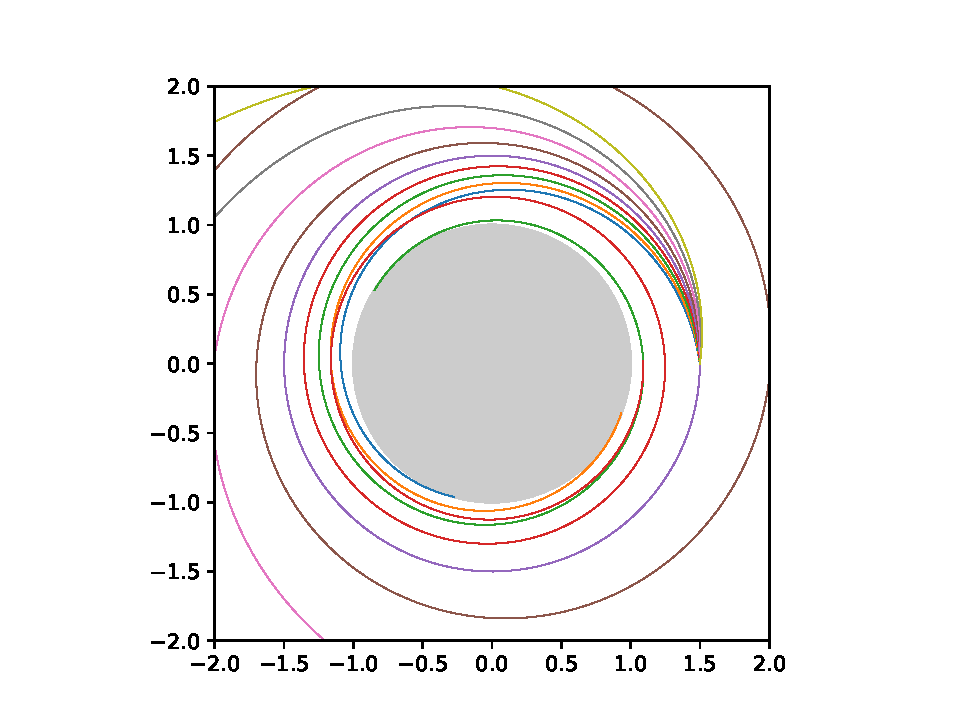
\includegraphics[width=\linewidth]{photon_trace.pdf}
\caption{The equatorial plane view of photon orbits. The photon emits from 1.5 $R_s$ (photon sphere) at different angles and orbits until it runs off the view or falls into the even horizon. Notice the photon sphere at 1.5 $R_s$}
\label{photon_trace}
\end{figure}
